\section{Information Gathering}

nformation gathering is an essential part of any security assessment. This is
the phase in which we gather all available information about the company, its
employees and infrastructure, and how they are organized. Information gathering
is the most frequent and vital phase throughout the penetration testing
process, to which we will return again and again.
\begin{figure}
  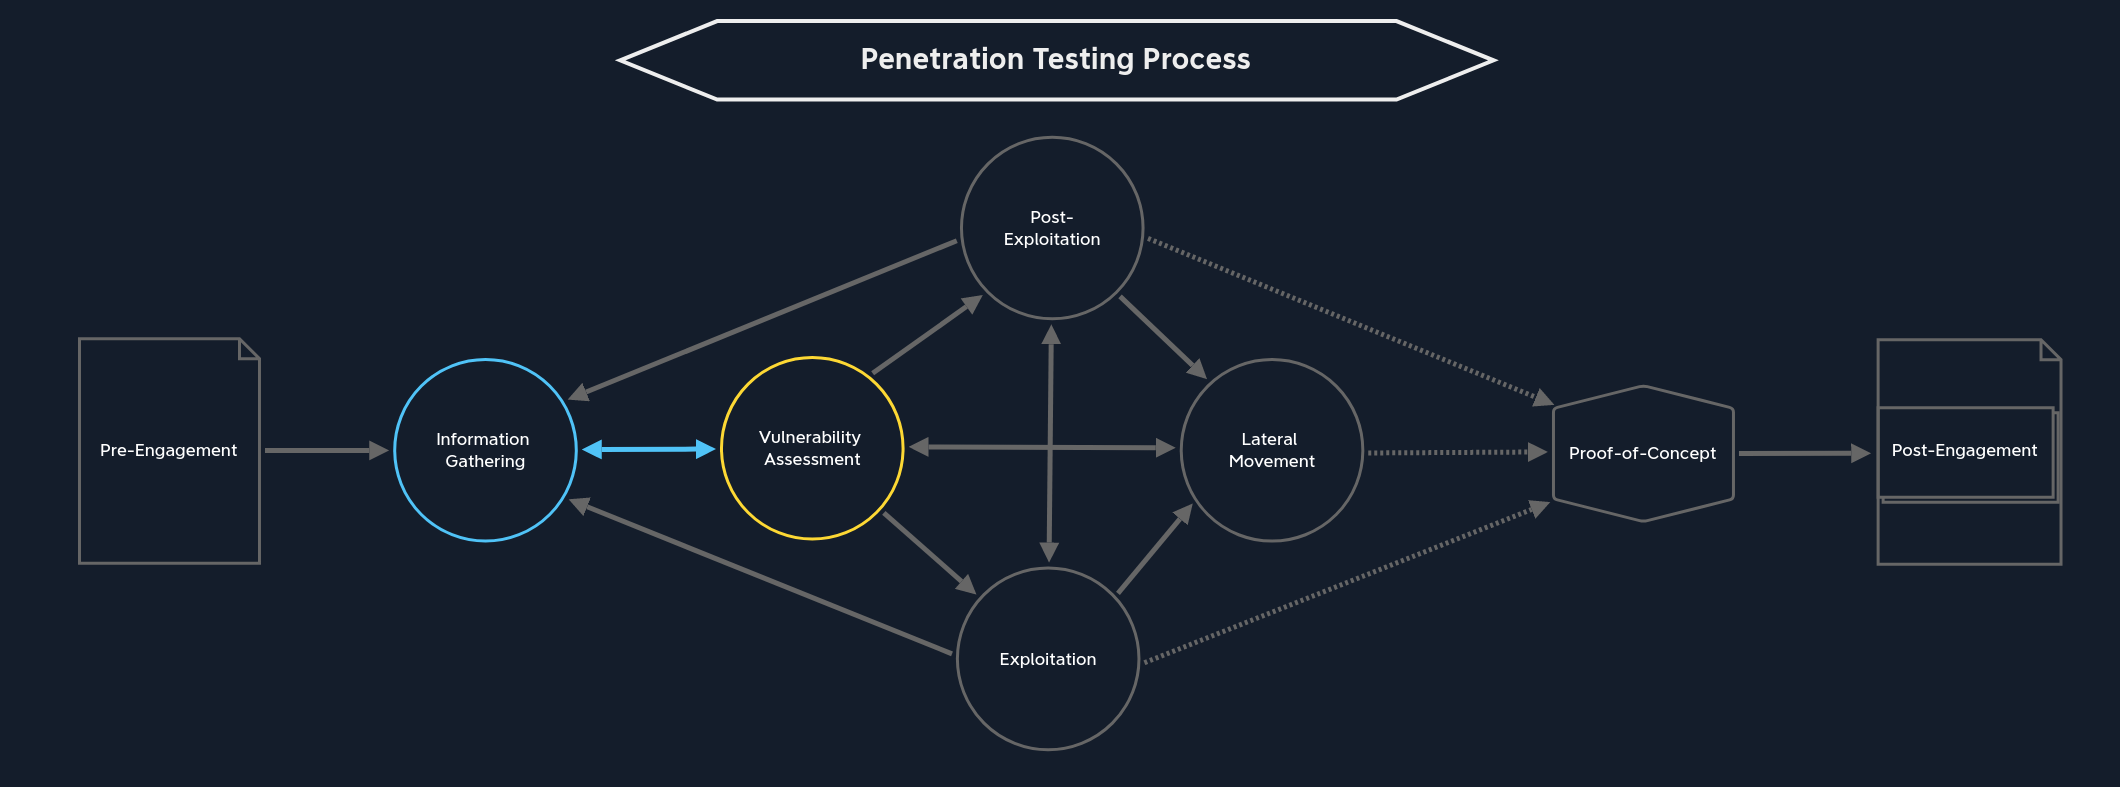
\includegraphics[width=\linewidth]{intro/process/images/int.png}
  \caption{Information gathering}
  \label{fig:pentest-process-info-gatehering}
\end{figure}
All the steps we take to exploit the vulnerabilities are based on the information we enumerate about our targets. This phase can be considered the cornerstone of any penetration test. We can obtain the necessary information relevant to us in many different ways. However, we can divide them into the following categories:
\begin{itemize}
    \item  Open-Source Intelligence
    \item  Infrastructure Enumeration
    \item  Service Enumeration
    \item  Host Enumeration
\end{itemize}

This is because the information is the main component that leads us to
successful penetration testing and identifying security vulnerabilities. We can
get this information anywhere, whether on social media, job postings,
individual hosts and servers, or even the employees. Information is continually
being spread and shared everywhere.


After all, we humans communicate by exchanging information, but network
components and services communicate similarly. Any exchange of information
always has a specific purpose. For computer networks, the aim is always to
trigger a particular process. Be it storing data in a database, registering,
generating specific values, or forwarding the information. 

\subsection{Open-Source Intelligence}
OSINT is a process for finding publicly available information on a target
company or individuals that allows the identification of events (i.e., public
and private meetings), external and internal dependencies, and connections.
OSINT uses public (Open-Source) information from freely available sources to
obtain the desired results. We can often find security-relevant and sensitive
information from companies and their employees. Usually, the people who share
such information are unaware that they are not the only ones who can access
it.

It is possible to find highly sensitive information such as passwords, hashes,
keys, tokens, and much more that can give us access to the network within just
a few minutes. Repositories on sites like Github or other development platforms
are often not set up correctly, and external viewers can see this information.
If this type of sensitive information is found at the onset of testing, the
Incident Handling and Report section of the RoE should describe the procedure
for reporting these types of critical security vulnerabilities. Publicly
published passwords or SSH keys represent a critical security gap if they have
not already been removed or changed. Therefore, our client's administrator must
review this information before we proceed.

Developers often share whole sections of code on StackOverflow to show other
developers a better overview of how their code works to help them solve their
problems. This type of information can also be found very quickly and used
against the company. Our task is to find such security holes and have them
closed.

\subsection{Infrastructure Enumeration}

During the infrastructure enumeration, we try to overview the company's
position on the internet and intranet. For this, we use OSINT and the first
active scans. We use services such as DNS to create a map of the client's
servers and hosts and develop an understanding of how their infrastructure is
structured. This includes name servers, mail servers, web servers, cloud
instances, and more. We make an accurate list of hosts and their IP addresses
and compare them to our scope to see if they are included and listed.

In this phase, we also try to determine the company's security measures. The
more precise this information is, the easier it will be to disguise our attacks
(Evasive Testing). But identifying firewalls, such as web application
firewalls, also gives us an excellent understanding of what techniques could
trigger an alarm for our customer and what methods can be used to avoid that
alarm.

Here, it also does not matter "where" we are positioned, whether we are trying
to gain an overview of the infrastructure from the outside (external) or
examining the infrastructure from the inside (internal) of the network.
Enumeration from inside the network gives us a good overview of the hosts and
servers that we can use as targets for a Password Spraying attack, in which we
use one password to attempt to authenticate with as many different user names
as possible, hoping for one successful authentication attempt to grant us a
foothold in the network. All these methods and techniques used for this purpose
will be looked at in more detail in the individual modules.

\subsection{Service Enumeration}

In service enumeration, we identify services that allow us to interact with the
host or server over the network (or locally, from an internal perspective).
Therefore, it is crucial to find out about the service, what version it is,
what information it provides us, and the reason it can be used. Once we
understand the background of what this service has been provisioned for, some
logical conclusions can be drawn to provide us with several options.

Many services have a version history that allows us to identify whether the
installed version on the host or server is actually up to date or not. This
will also help us find security vulnerabilities that remain with older versions
in most cases. Many administrators are afraid to change applications that work,
as it could harm the entire infrastructure. Therefore, administrators often
prefer to accept the risk of leaving one or more vulnerabilities open and
maintaining the functionality instead of closing the security gaps.

\subsection{Host Enumeration}

Once we have a detailed list of the customer's infrastructure, we examine every
single host listed in the scoping document. We try to identify which operating
system is running on the host or server, which services it uses, which versions
of the services, and much more. Again, apart from the active scans, we can also
use various OSINT methods to tell us how this host or server may be
configured.

We can find many different services, such as an FTP server that the company
uses to exchange data between employees and even allows anonymous access. Even
today, there are many hosts and servers that the manufacturers no longer
support. However, vulnerabilities are still found for these older versions of
operating systems and services, which then remain and endanger our client's
entire infrastructure.

It does not matter here whether we examine each host or server externally or
internally. However, from the internal perspective, we will find services that
are often not accessible from the outside. Therefore, many administrators
become careless and often consider these services "secure" because they are not
directly accessible from the internet. Thus, many misconfigurations are often
discovered here due to these assumptions or lax practices. During host
enumeration, we try to determine what role this host or server plays and what
network components it communicates with. In addition, we must also identify
which services it uses for this purpose and on which ports they are located.

During internal host enumeration, which in most cases comes after the
successful Exploitation of one or more vulnerabilities, we also examine the
host or server from the inside. This means we look for sensitive files, local
services, scripts, applications, information, and other things that could be
stored on the host. This is also an essential part of the Post-Exploitation
phase, where we try to exploit and elevate privileges.

\subsection{Pillaging}

Another essential step is Pillaging. After hitting the Post-Exploitation stage,
pillaging is performed to collect sensitive information locally on the already
exploited host, such as employee names, customer data, and much more. However,
this information gathering only occurs after exploiting the target host and
gaining access to it.

The information we can obtain on the exploited hosts can be divided into many
different categories and varies greatly. This depends on the purpose of the
host and its positioning in the corporate network. The administrators taking
the security measures for these hosts also play a significant role.
Nevertheless, such information can show the impact of a potential attack on our
client and be used for further steps to escalate our privileges or move
laterally further in the network.
